\documentclass[12pt, twoside]{article}
\usepackage[letterpaper, margin=1in, headsep=0.5in]{geometry}
\usepackage[english]{babel}
\usepackage[utf8]{inputenc}
\usepackage{amsmath}
\usepackage{amsfonts}
\usepackage{amssymb}
\usepackage{tikz}
\usetikzlibrary{quotes, angles}
\usepackage{graphicx}
\usepackage{enumitem}
\usepackage{multicol}

\newif\ifmeta
\metatrue %print standards and topics tags

\title{Regents Geometry}
\author{Chris Huson}
\date{September 2020}

\usepackage{fancyhdr}
\pagestyle{fancy}
\fancyhf{}
\renewcommand{\headrulewidth}{0pt} % disable the underline of the header
\raggedbottom


\fancyhead[LE]{\thepage}
\fancyhead[RO]{\thepage \\ Name: \hspace{4cm} \,\\}
\fancyhead[L]{BECA / Dr. Huson / Geometry 05-Transformations\\* pset ID: 70}

\begin{document}

\subsubsection*{5-9PreExam-Transformations}
\begin{enumerate}
\item Apply a rotation of $90^\circ$ centered at the origin to $\triangle ABC$. Plot and label the image on the axes below and make a table of its coordinates.
  \begin{flushright}
    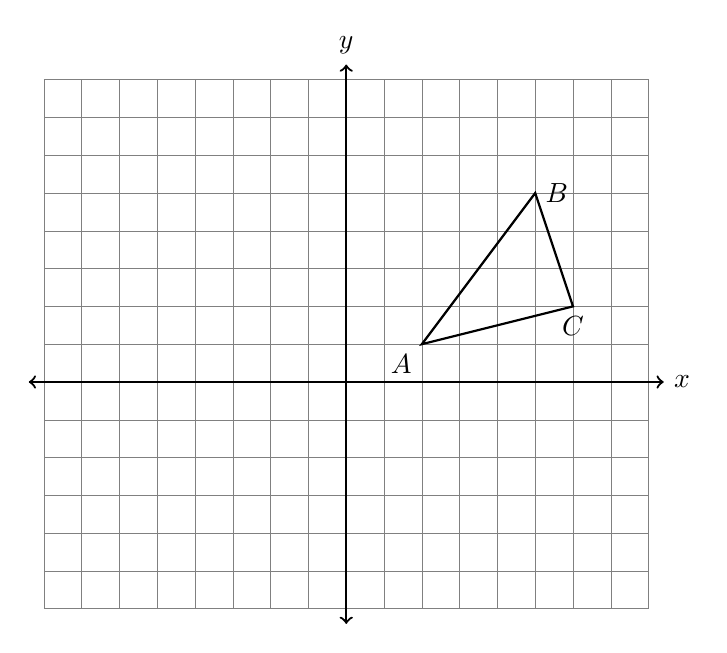
\begin{tikzpicture}[scale=.48]
      \draw [help lines] (-8,-6) grid (8,8);
      \draw [thick, <->] (-8.4,0) -- (8.4,0) node [right] {$x$};
      \draw [thick, <->] (0,-6.4)--(0,8.4) node [above] {$y$};
      \draw [thick]
        (2,1) node[below left] {$A$}--
        (5,5) node[right] {$B$}--
        (6,2) node[below] {$C$}--
        cycle;
    \end{tikzpicture}
  \end{flushright}

\item The vertices of $\triangle JKL$ have the coordinates $J(-4,-2)$, $K(-1,-1)$, and $L(-2,3)$, as shown below. \\[0.25cm]
  Apply a translation of $(x,y) \rightarrow (x-3, y+2)$ to $\triangle JKL$ and then reflect the image across the $y$-axis. Draw both images $\triangle J'K'L'$ and $\triangle J''K''L''$ on the set of axes below, labeling the vertices.
  \begin{flushright}
    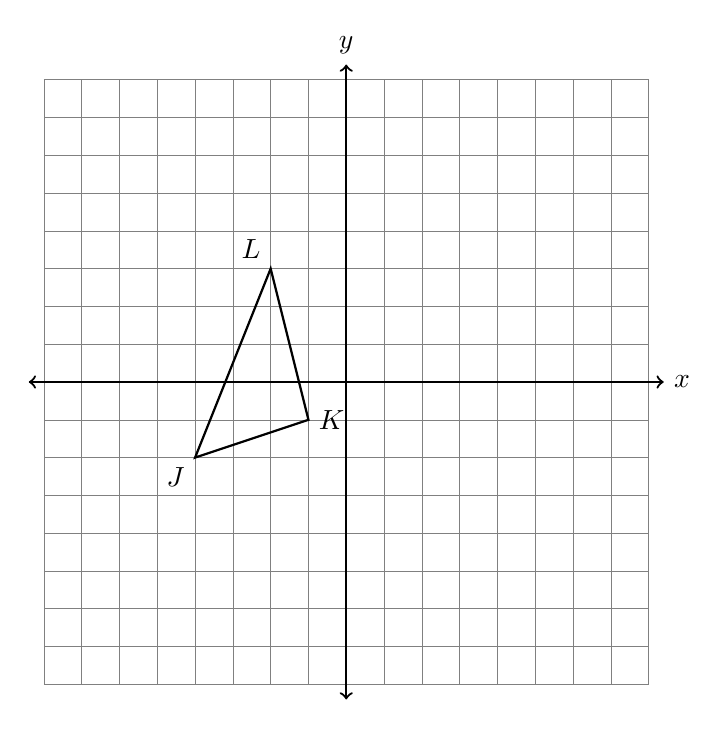
\begin{tikzpicture}[scale=.48]
      \draw [help lines] (-8,-8) grid (8,8);
      \draw [thick, <->] (-8.4,0) -- (8.4,0) node [right] {$x$};
      \draw [thick, <->] (0,-8.4)--(0,8.4) node [above] {$y$};
      \draw [thick]
        (-4,-2) node[below left] {$J$}--
        (-1,-1) node[right] {$K$}--
        (-2,3) node[above left] {$L$}--
        cycle;
    \end{tikzpicture}
  \end{flushright}

  \newpage
\item Find the area of the parallelogram $ABCD$ shown below, with $AB=9.5$ and height $h=7.1$.
  \begin{flushright}
  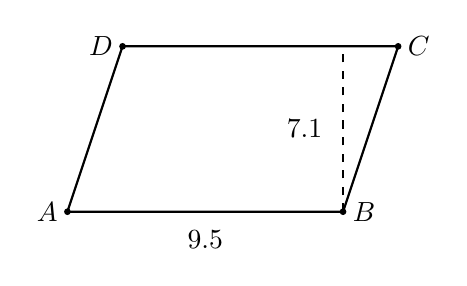
\begin{tikzpicture}[scale=0.7]
    \draw [-, thick] (0,0)--(5,0)--(6,3)--(1,3)--cycle;
    \draw [-, dashed] (5,0)--(5,3);
    \draw [fill] (0,0) circle [radius=0.05] node[left]{$A$};
    \draw [fill] (5,0) circle [radius=0.05] node[right]{$B$};
    \draw [fill] (6,3) circle [radius=0.05] node[right]{$C$};
    \draw [fill] (1,3) circle [radius=0.05] node[left]{$D$};
    \node at (4.3, 1.5){$7.1$};
    \node at (2.5, -0.5){9.5};
  \end{tikzpicture}
  \end{flushright}

\item Find the sum of the measures of the internal angles of a hexagon. Show the formula.  \vspace{3cm}

\item  A wooden cutting board is $8 \frac{1}{2}$ inches long, 7 inches wide, and $1 \frac{1}{4}$ inches thick. Find the volume of the box. Show the calculation.
\begin{flushright}
  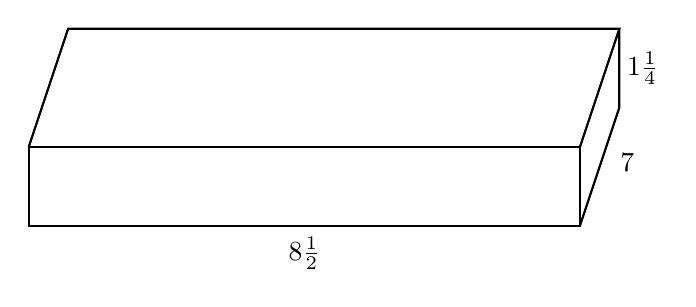
\begin{tikzpicture}[scale=1]
    \draw [-, thick] (0,0)--(7,0)--(7,1)--(0,1)--cycle;
    \draw [-, thick] (0,1)--(0.5,2.5)--(7.5,2.5)--(7,1);
    \draw [-, thick] (7,0)--(7.5,1.5)--(7.5,2.5);
    \node at (7.8, 2){$1 \frac{1}{4}$};
    \node at (3.5, -0.35){$8 \frac{1}{2}$};
    \node at (7.6, 0.8){$7$};
  \end{tikzpicture}
  \end{flushright} \vspace{3cm}

\item Of two complementary angles, the measure of $\angle A$ is two times that of $\angle B$. Find $m\angle A$. \vspace{3.5cm} 

\newpage


\item An angle bisector is shown below, with $\overrightarrow{AC}$ bisecting $\angle BAD$. Given $m\angle BAC = 6x-5$ and $m\angle BAD = 9x+17$, find $m\angle BAD$. (Show check)
\begin{flushright}
\begin{tikzpicture}[scale=0.7, rotate=30]
  \draw [<->, thick] (100:7)node[left]{$B$} 
  --(0,0)node[below]{$A$}
  --(6,0)node[below]{$D$}--(7,0);
  \draw [->, thick] (0,0)--(50:7)node[below right]{$C$};
  %\draw [fill] (0,0) circle [radius=0.05] node[below]{$A$};
  %\draw [fill] (5,0) circle [radius=0.05] node[below]{$B$};
\end{tikzpicture}
\end{flushright} \vspace{3cm}

\item Angles $APC$ and $CPD$ form a linear pair. $m\angle APC = 10x-10$ and $m\angle CPD = 3x-5$. Find $m\angle CPD$. Check your answer for full credit.
  \begin{flushright}
    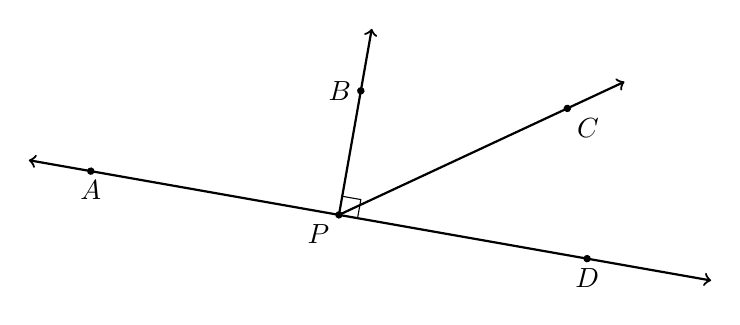
\begin{tikzpicture}[scale=0.8, rotate=-10]
      \draw [->, thick] (0,0)--(35:5);
      \draw [<->, thick] (-5,0)--(6,0);
      \draw [->, thick] (0,0)--(0,3);
      \draw (0,0)++(0.3,0)--++(0,0.3)--+(-0.3,0);
      %\draw [fill] (-1,2.5) circle [radius=0.05] node[left ]{$B$};
      \draw [fill] (35:4) circle [radius=0.05] node[below right]{$C$};
      \draw [fill] (-4,0) circle [radius=0.05] node[below]{$A$};
      \draw [fill] (0,0) circle [radius=0.05] node[below left]{$P$};
      \draw [fill] (0,2) circle [radius=0.05] node[left]{$B$};
      \draw [fill] (4,0) circle [radius=0.05] node[below]{$D$};
    \end{tikzpicture}
    \end{flushright}
    \vspace{5cm}

\newpage

\subsubsection*{Do Not Solve! \\
Model the situation with an equation in terms of $x$.}

\item Given $\overline{ABC}$, with $AB=2x-1$, $BC=3x+7$, and $AC=21$. Find $x$. \vspace{1cm}
  \begin{flushright}
    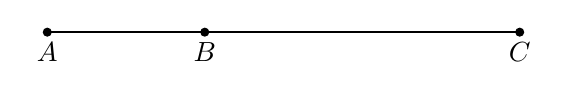
\begin{tikzpicture}
      \draw [-, thick] (0,0) node[below]{$A$}--
      (2,0) node[below]{$B$}--
      (6,0) node[below]{$C$};
      \draw [fill] (0,0) circle [radius=0.05];
      \draw [fill] (2,0) circle [radius=0.05];
      \draw [fill] (6,0) circle [radius=0.05];
    \end{tikzpicture}
    \end{flushright} \vspace{1cm}
  
\item Given $m\angle 3 = x+35$ and $m\angle 5 = 4x-25$. Find $x$. 
  \begin{flushright}
  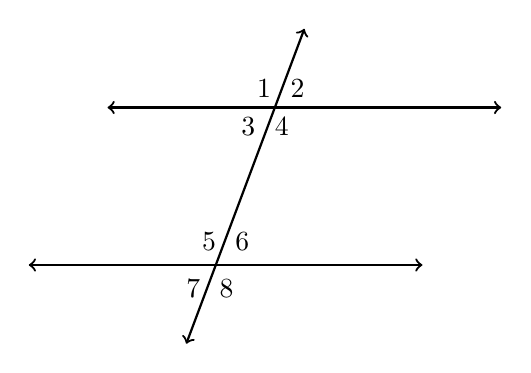
\begin{tikzpicture}
    \draw [<->, thick] (3,2)--(8,2);
    \draw [<->, thick] (2,0)--(7,0);
    \draw [<->, thick] (4,-1)--(5.5,3);
    \node at (4.5,0.3) [left]{$5$};
    \node at (4.5,0.3) [right]{$6$};
    \node at (4.3,-0.3) [left]{$7$};
    \node at (4.3,-0.3) [right]{$8$};
    \node at (5.2,2) [above left]{$1$};
    \node at (5.2,2) [above right]{$2$};
    \node at (5,2) [below left]{$3$};
    \node at (5,2) [below right]{$4$};
  \end{tikzpicture}
  \end{flushright} \vspace{0.5cm}

\item In the diagram below $m\angle AOB = 6x+5$ and $m\angle COB = 8x+15$. Find $x$. %\vspace{0.25cm}
  \begin{flushright}
  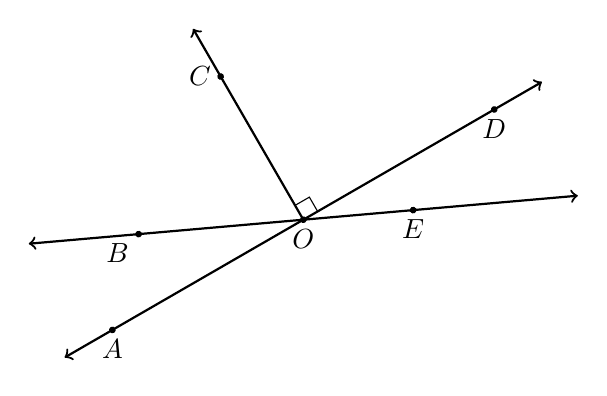
\begin{tikzpicture}[scale=0.7, rotate=30]
  \draw [<->, thick] (-25:5)--(0,0)--(155:5);
  \draw [<->, thick] (-5,0)--(5,0);
  \draw [->, thick] (0,0)--(0,4);
  \draw (0,0)++(0.3,0)--++(0,0.3)--+(-0.3,0);
  %\draw [fill] (-1,2.5) circle [radius=0.05] node[left ]{$B$};
  \draw [fill] (155:3) circle [radius=0.05] node[below left]{$B$};
  \draw [fill] (-4,0) circle [radius=0.05] node[below]{$A$}; 
  \draw [fill] (0,0) circle [radius=0.05] node[below]{$O$};
  \draw [fill] (0,3) circle [radius=0.05] node[left]{$C$};
  \draw [fill] (4,0) circle [radius=0.05] node[below]{$D$};
  \draw [fill] (-25:2) circle [radius=0.05] node[below]{$E$};
  \end{tikzpicture}
  \end{flushright}

\item The point $K$ is the midpoint of $\overline{JL}$, $JK=3x+15$, and $JL=9x+9$. Find $x$.  \vspace{1cm}
  \begin{flushright}
    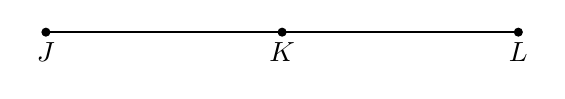
\begin{tikzpicture}
      \draw [-, thick] (0,0) node[below]{$J$}--
      (3,0) node[below]{$K$}--
      (6,0) node[below]{$L$};
      \draw [fill] (0,0) circle [radius=0.05];
      \draw [fill] (3,0) circle [radius=0.05];
      \draw [fill] (6,0) circle [radius=0.05];
    \end{tikzpicture}
    \end{flushright} \vspace{2cm}

\newpage
\item The measures in degrees of the three angles of a triangle are $3x$, $\frac{1}{2}x+7$, and $5x-65$. Find $x$. \vspace{4cm}


\newpage

\item Given $\overleftrightarrow{RS}$ as shown on the number line, with $R=-3.3$ and $S=5.1$. \\[20pt] % Midpoint
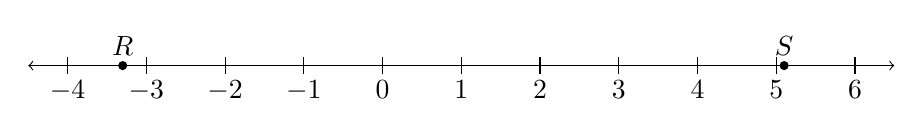
\begin{tikzpicture}
  \draw [<->] (-4.5,0)--(6.5,0);
  \foreach \x in {-4,...,6} %2 leading for diff!=1
    \draw[shift={(\x,0)},color=black] (0pt,-3pt) -- (0pt,3pt) node[below=5pt]  {$\x$};
    \draw [fill] (-3.3,0) circle [radius=0.05] node[above] {$R$};
    \draw [fill] (5.1,0) circle [radius=0.05] node[above] {$S$};
\end{tikzpicture}
\begin{enumerate}
  \item What is the exact distance on the number line between the points $R$ and $S$? \vspace{3cm} 
  \item The point $T$ bisects $\overline{RS}$. Find the value of $T$, and mark and label it on the numberline $\overleftrightarrow{RS}$ shown above. 
\end{enumerate} \vspace{3cm} 


\item The trapezoid $ABCD$ has two parallel sides, $\overline{AB} \parallel \overline{CD}$ with lengths $AB=9$ and $CD=11$. The trapezoid's height is $h=7.25$. Find the area of the trapezoid. \\[0.25cm]
  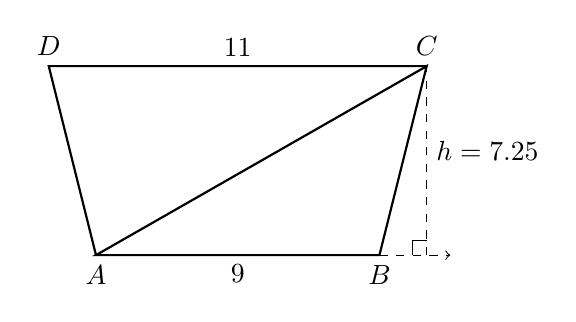
\begin{tikzpicture}[scale=0.6]
    \draw [thick]
      (0,0)node[below]{$A$}--
      (6,0)node[below]{$B$}--
      (7,4)node[above]{$C$} --cycle;
    \draw [thick] (0,0)--(-1,4)node[above]{$D$}--(7,4);
    \draw [dashed] (7,0)--(7,4);
    \draw [dashed, ->] (6,0)--(7.5,0);
    \draw (7,0)++(-0.3,0)--++(0,0.3)--+(0.3,0);
    \node at (7,2.2)[right]{$h=7.25$};
    \node at (3,0)[below]{$9$};
    \node at (3,4)[above]{$11$};
  \end{tikzpicture} \vspace{2cm}

\item Find the area of $\triangle KAT$. The altitude $h$ of the triangle is 11.0 centimeters and the base $KA=19.6$ cm. Show work by writing an equation before making the calculation.
  \begin{flushright}
    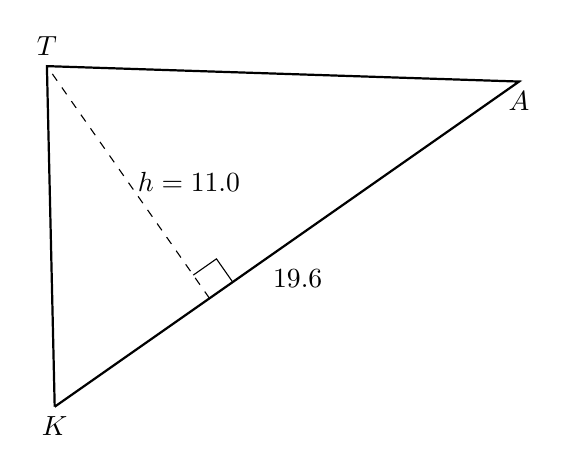
\begin{tikzpicture}[scale=1.2, rotate=35]
      \draw [thick]
        (2,0)node[below]{$K$}--
        (8,0)node[below]{$A$}--
        (4,3)node[above]{$T$} --(2,0);
    \draw [dashed] (4,0)--(4,3);
    \draw (4,0)++(0.3,0)--++(0,0.3)--+(-0.3,0);
    \node at (4,1.5)[right]{$h=11.0$};
    \node at (5,-0.2)[below]{$19.6$};
    \end{tikzpicture} 
  \end{flushright} \vspace{1.0cm}

\newpage

\item A feeding trough in the shape of a rectangular prism is 105 inches long. The trough's cross section is square. If its volume is 15,120 cubic inches, what is the dimension of each side of its square end, $x$? (drawing not to scale)
  \begin{flushright}
    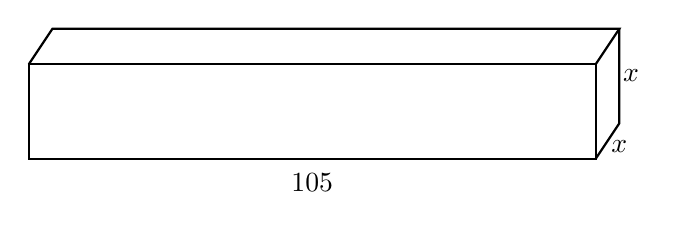
\begin{tikzpicture}[scale=.6]
      \draw [-, thick] (0,0)--(12,0)--(12,2)--(0,2)--cycle;
      \draw [-, thick] (0,2)--(0.5,2.75)--(12.5,2.75)--(12,2);
      \draw [-, thick] (12,0)--(12.5,0.75)--(12.5,2.75);
      \node at (12.75, 1.75){$x$};
      \node at (6, -0.5){$105$};
      \node at (12.5, 0.25){$x$};
    \end{tikzpicture}
    \end{flushright} \vspace{5cm}

\item Given $\overrightarrow{BA} \perp \overrightarrow{BC}$, $m \angle ABD = 2x$, and $m \angle DBC = x-15$. Find $m \angle DBC$. \\[0.25cm]
  For full credit, show the check using both angle measures.
    \begin{flushright}
    \begin{tikzpicture}[scale=1.2]
      \draw [<->, thick] (0,3) node[left]{$A$}--
        (0,0) node[below]{$B$}--
        (4,0) node[below]{$C$};
      \draw [->, thick] (0,0)--(20:3.5) node[above left]{$D$};
      \draw [-, thin] (0, 0.4)--(0.4, 0.4)--(0.4, 0);
    \end{tikzpicture}
    \end{flushright}
    \vspace{1cm}


\newpage

\item Given parallel lines $\overleftrightarrow{AB} \parallel \overleftrightarrow{CDE}$ with $\overline{AD} \cong \overline{CD}$. If $m\angle 1=78$ find $m\angle 2$.
  \begin{flushright}
  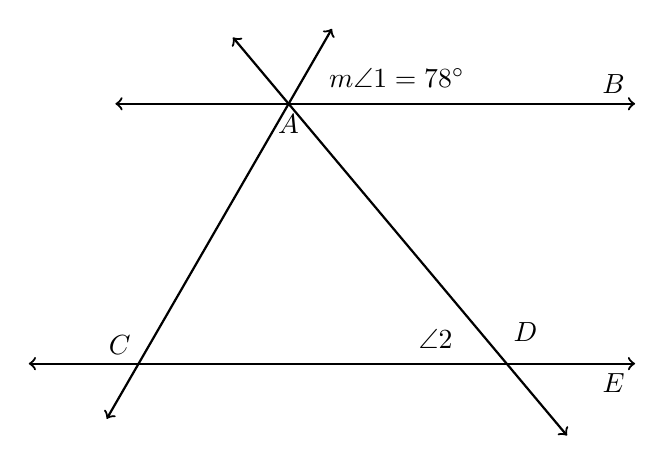
\begin{tikzpicture}[scale=1.1]
    \draw [<->, thick] (-2,0)--(4,0) node[above left]{$B$};
    \draw [<->, thick] (-3,-3)--
      (4,-3) node[below left]{$E$};
    \draw [<->, thick] (-120:4.2)--
      (0,0) node[below]{$A$}--(60:1);
    \draw [<->, thick] (130:1)--(-50:5);
    \node at (1.25, 0.3){$m\angle 1=78^\circ$};
    \node at (-44:3.8){$D$};
    \node at (-125:3.4){$C$};
    \node at (-58:3.2){$\angle 2$};
  \end{tikzpicture}
  \end{flushright} \vspace{4cm}

\item The volume of the rectanglar prism shown is 120 cubic feet. Its length is length is ten feet longer than its height $x$. Its depth is 5 feet. Find the length of the prism. \\(not drawn to scale)
  \begin{flushright}
    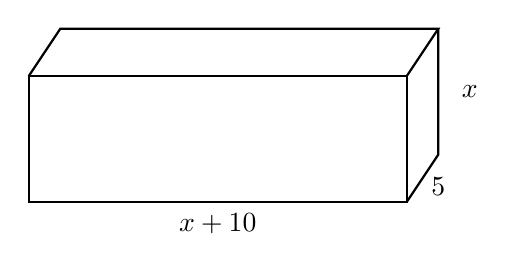
\begin{tikzpicture}[scale=0.8]
      \draw [-, thick] (0,0)--(6,0)--(6,2)--(0,2)--cycle;
      \draw [-, thick] (0,2)--(0.5,2.75)--(6.5,2.75)--(6,2);
      \draw [-, thick] (6,0)--(6.5,0.75)--(6.5,2.75);
      \node at (7, 1.75){$x$};
      \node at (3, -0.35){$x+10$};
      \node at (6.5, 0.25){$5$};
    \end{tikzpicture}
    \end{flushright} \vspace{3cm} 

\end{enumerate}
\end{document}